
A picture is worth a thousand words – especially when you are trying to understand and gain insights from data. It is particularly relevant when you are trying to find relationships among hundreds, or even thousands, of variables to determine their relative importance.
\section{Conventional Data Visualization Methods}
Many conventional data visualization methods are often used. They are: table, histogram, scatter plot, line chart, bar chart, pie chart, area chart, flow chart, bubble chart, time line, Venn diagram, data flow diagram, and entity relationship diagram, etc. In addition, some data visualization methods have been used although they are less known compared the above methods. The additional methods are: parallel coordinates, treemap, cone tree, and semantic network, etc.
\par
There are many conventional data visualization techniques which are focused in this document because these techniques have generic features and common understanding. These data presentation should be beautiful, elegant, descriptive, and interpretable in order to convey message to the reader effectively. There are new developed fascinating methods are introducing, but modern approaches have its own implementation problems and no commonality, so difficult to adopt. Data visualization represents data in the way that simplifies data interpretation and its relationship.
\subsection{Pie Chart}
A pie chart is also called circle graph. Pie chart circle is divided into number of sectors, each circle describe a proportion in a whole quantity. The pie chart control is use to determines the size of data wedge as compare to other data wedges. In pie chart a wedge represents the part of data that has common feature or characteristics. Wedges can be labeled to identify different data points. Most of the time is shown in percentage.
\begin{figure}[h]
	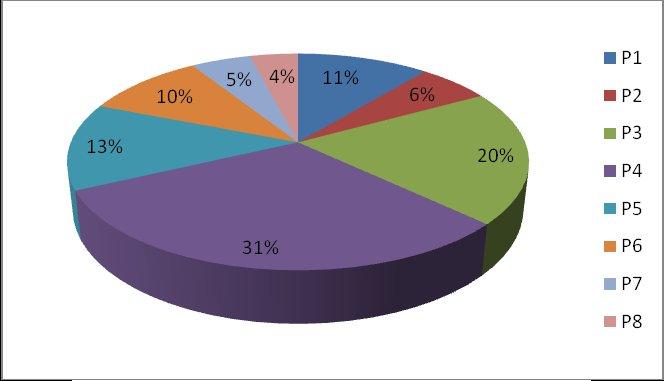
\includegraphics[width=4cm, height=4cm]{piechart}
	\centering
	\caption{Standard Pie Chart}
\end{figure}.
\subsection{Bar Chart}
One of the most commonly use data visualization method is bar chart, it is also called Bar Graph(also called Column chart). Bar chart is most of the time use for discrete data not for continuous data. Bar Chart control has been use to represent data in horizontal bars, the vertical length of the bar represent the values. Bar chart is use to represent a single data series and related data points are group in one series. For example monthly salaries, it can be mutli bar graph i.e. percentage increase per month as shown in the following figure.

\begin{figure}[h]
	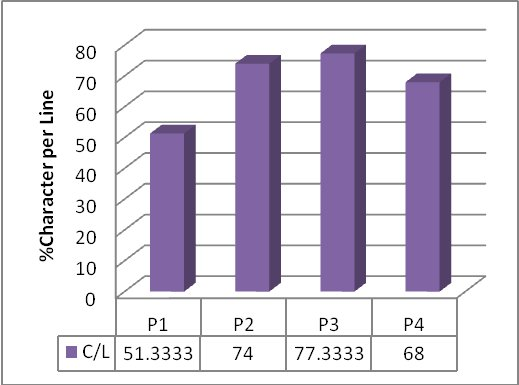
\includegraphics[width=4cm, height=4cm]{barchart}
	\centering
	\caption{Bar Chart}
\end{figure}
\subsection{Line Chart}
Line chart is common well known graph in many fields, also label as line graph. It is a graph which is use to display information in connected points. These points are connected through continuous or straight line. Line graph is the extension of Scatter plot. Data points can be represented by icons or symbols, or can also draw simple line without icons
\begin{figure}[h]
	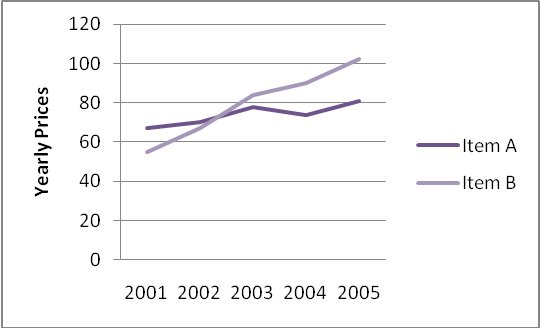
\includegraphics[width=4cm, height=4cm]{linechart}
	\centering
	\caption{Line Chart}
\end{figure}
\subsection{Area Chart}
Area chart is also called area graph, use to display quantitative data graphically. Area chart control is use represent data in bounded area. The bounded area is based on the line graph, the line is generated and the area below is shaded with colors,different texture and hatching, which produce area graph.
\begin{figure}[h]
	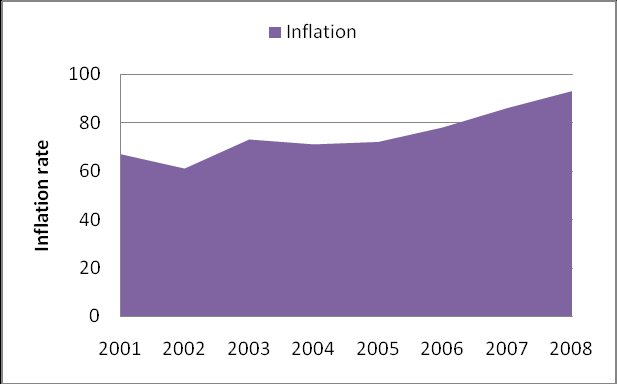
\includegraphics[width=4cm, height=4cm]{areachart}
	\centering
	\caption{Area Chart}
\end{figure}
\subsection{Scatter Plot}
Scatter Plot is also known as plot, plot chart, scatter chart, scattergram, scatter diagram or scatter graph. Scatter plot is graphical display of set of data in Cartesian coordinate, shows the relationship between two variables, one variable represent horizontal distance (independent variable) and second variable vertical distance (dependent variable) of data point from the coordinate axis. Scatter plot shows the how strong the relationship are between the variables, and determines whether their exit any outlier in the data or not. It is use to look how the data is dispersed.
\begin{figure}[h]
	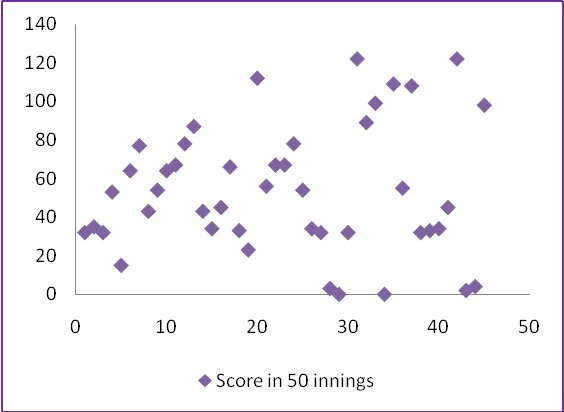
\includegraphics[width=4cm, height=4cm]{scatterplot}
	\centering
	\caption{Scatter Plot Diagram}
\end{figure}

\section{Interactive Visualization}
The users are interested in the abstract data about which they have desire to understand, the user don’t have sufficient pre knowledge about that data. Hence for the exploration, analysis, and for the representation of data or information visualization interactive techniques are exceptionally momentous. The challenge in information visualization is to provide data visually in order to the user effectively understand the information for which the user is looking for, for this purpose provide interaction mechanism that make is possible to manipulate visualization effectively and effortlessly as probable. Users can interact with interfaces or visualization in different ways by means of mouse over, single click, double click, or can add multiple interactive options by mouse right button click. There are many interactive techniques available to interact with charts or graphical representation to understand the drill down details. Card et al introduce the interactive mechanism of visualization in 1999.
\par
Interactive visualization can be performed through approaches such as zooming (zoom in and zoom out), overview and detail, zoom and pan, and focus and context or fish eye. The steps for interactive visualization are as follows:
\subsection{Selecting}
One of the most important and fundamental requirements in visualization is interactive selection of data entities or subset or part of whole data or whole data set, that is of interest to the user. This is useful to view detail information about the selected entities, highlight entities that are covered or hidden, cluster entities that are related and extracting entities that may be use in future.
\subsection{Linking}
Linking and brushing are the most common form of linking. Linking is useful to relate information among multiple views. Information can be mapped differently to different views to reveal or expose different perspectives (viewpoint) or different portions of the information. On the bases of selection criteria the user can select entities in one structure, which then shows the distribution the selected entities in another structure.
\subsection{Filtering}
Filtering enables users to dynamically adjust amount of information to display, means to decrease or increase information quantity that need to display, and focus on information of interest. For this purpose need some dynamic query values to manipulate, in this regard visual widgets can play vital role e.g. slider can be use in different ranges, field box can be use to put attribute value in specified range etc.These widgets enables one from the current query parameters and enables to quickly adjust query parameters and instantaneously view filtered results in the visualization in real time.
\subsection{Rearranging or Remapping}
As a single mapping or plotting visual form of information may be not enough, so the users must empower to customize mapping among many maps. To enable users to customize maps by its own choice provide the way to better understand the information. As the spatial layout is the most important visual mapping, rearranging the spatial layout of the information is the most effective for producing different insights
\begin{figure}[h]
	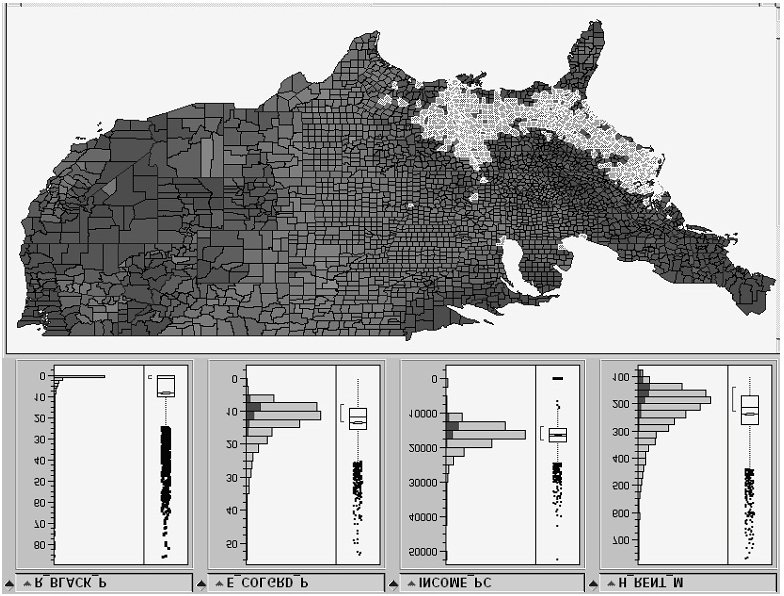
\includegraphics[width=\textwidth, height=8cm]{interactivebrushing}
	\centering
	\caption{Interactive brushing and linking between histogram plots (top) and geographic map (bottom) of datasets}
\end{figure}
\section{Data Visualization Tools}
Following are the most awesome data visualization tools available on the web
\begin{multicols}{3}
\begin{itemize}
	\item Dygraph
	\item ZingCharts
	\item InstantAtlas
	\item Timeline
	\item Exhibit
	\item Modest Maps
	\item Leaflet
	\item WolframAlpha
	\item Visual.ly
	\item VisualizeFree
	\item Better World Flux
	\item Fusion Charts
	\item jqPlot
	\item Dipity
	\item Many Eyes
	\item D3.js
	\item jpGraphs
	\item HighCharts
	\item Google Charts
	\item CrossFilter
\end{itemize}
\end{multicols}
